%--------1---------2---------3---------4---------5---------6---------7---------8---------9---------1---------2---------3---------4---------5---------6
%23456789 123456789 123456789 123456789 123456789 123456789 123456789 123456789 123456789 123456789 123456789 123456789 123456789 123456789 123456789

\glsunsetall
\chapter{Estimating the random error in a \texorpdfstring{\gls{AUCXIC}}{peak-area} fraction given only one run}
\label{chap:error}
\glsresetall

\begin{figure}[tpbh]
\small
\begin{framed}
\begin{center}
\begin{tikzpicture}
\begin{axis}[
	ticks=none, align=center, width=0.8\textwidth, height=0.33\textheight,
	title={Part of the 3D-chromatogram of one run of \gls{LC-MS/MS} \\
			in which \(X\) is the \gls{AUCXIC} of a product-ion \(A\) and \(Y\) is the \gls{AUCXIC} of a product-ion \(B\) \\
			such that \(B\) is chemically different from \(A\)},
		xlabel=\glsfirst{RT},
		ylabel=\glsfirst{m/z},
	  zlabel=\text{Absolute intensity}]
		\addplot3[surf,samples=25,samples y=8,shader=interp,domain=-3:3] 
		{1.5 * exp(0-0.5*x^2) * exp(0-6*(y-1.5)^2) + exp(0-0.5*x^2) * exp(0-6*(y+1.5)^2)};
  \node[coordinate,pin=above:{\(X\)}] 
  		at (axis cs:0,-1.5) {};
  \node[coordinate,pin=above:{\(Y\)}] 
  		at (axis cs:0,1.5)	{};
  \node[coordinate,pin=above:{\(\displaystyle\frac{X}{X+Y}\approx\frac{2}{5}\pm?\)}] 
    		at (axis cs:1.5,3.5)	{};
\end{axis}
\end{tikzpicture}
\end{center}
Our objective is to estimate the random error in \(\frac{X}{X+Y}\) from only one run of \gls{LC-MS/MS}.
\(\frac{X}{X+Y}\) represents the quantity of \(A\) relative to \(B\).
\end{framed}
\caption[
	The graphical abstract of \cref{chap:error}.]{
	The graphical abstract of \cref{chap:error} (hypothetical data used as example).
  \label{fig:error:graphical-abstract}}
\end{figure}
\clearpage

For any run of \gls{LC-MS} or of \gls{LC-MS/MS}, the \gls{AUCXIC} of a chemical species is defined as the area under the curve of the \gls{XIC} of this chemical species.
This \gls{AUCXIC} represents the total quantity of this chemical species detected in this run of \gls{LC-MS} or of \gls{LC-MS/MS}. 
\Gls{AUCXIC} fraction of a first chemical species relative to a second chemical species is defined as follows:
	the \gls{AUCXIC} of this first chemical species, divided by the sum of the \gls{AUCXIC} of this first chemical species and the \gls{AUCXIC} of this second chemical species.		

Multiple repeated runs can empirically estimate the random error in a measurement of \gls{AUCXIC} fraction.
Given only one run, this random error seems to be impossible to estimate, because the sample variance of every sample of size one is undefined.
However, from some assumptions that are partially supported by evidence in the literature,
	we mathematically deduced an empirical formula that estimates this random error.
We extracted more than 10000 \gls{AUCXIC} fractions from a test dataset produced by three runs of \gls{LC-MS/MS}.{}
Then, for each \gls{AUCXIC} fraction in these \gls{AUCXIC} fractions and for each applicable run among these three runs,
	our empirical formula predicted the variance in the single measurement of this \gls{AUCXIC} fraction.{}
Then, we compared such predicted variances with the sample variances respectively observed in some pairs of nearly repeated runs.
This comparison confirms the following.
Each of these \gls{AUCXIC} fractions empirically follows the normal distribution with such corresponding predicted variance.
Thus, our empirical formula can estimate the random error in one single measurement of \gls{AUCXIC} fraction.
	
Our empirical formula cannot offer every benefit that multiple repeated runs can offer.{}
For example, multiple repeated runs can respectively provide multiple estimates of the mean of a \gls{AUCXIC}, 
	and the average of these estimates is a more precise estimate of this mean.
Moreover, the test dataset is produced by only one \gls{QTOF} mass spectrometer analyzing only one non-complex sample.
%Thus, our empirical formula may not be applicable to a dataset 
%produced by an arbitrary mass spectrometer on an arbitrary sample.
However, 
	the more similar a second experiment is to the experiment that produced the test dataset,
	the more applicable our empirical formula is to the dataset produced by this second experiment.{}
Fortunately, the same mass spectrometer produced both the \gls{MS/MS} dataset and the test dataset, 
	and two similar samples respectively generated these two datasets.{}
Thus, our empirical formula is very applicable to the \gls{MS/MS} dataset used in \cref{chap:oxlvl}.
Thus, \cref{chap:oxlvl} uses \cref{eq:NM:derivation:simplificationresult}, a key result of this chapter,
	for estimating the confidence in our quantitation of oxidation. %and thus the confidence in our characterization of \gls{SASA}.{}
More specifically, for the y-ions that have the same residue sequence and thus the same y-ion index,
	the \gls{AUCXIC} fraction of oxidized y-ions over both oxidized or unoxidized y-ions is the fraction of oxidation that occurred before this y-ion index.
Thus, \cref{chap:oxlvl} uses such \gls{AUCXIC} fraction to quantitate the extent of oxidation at subpeptide level.
		
\section{Motivation}
\label{sec:error:motivation}

This chapter provides an empirical formula for the following purpose: 
	estimating the random error in a \gls{AUCXIC} fraction that is measured once in only one run of \gls{LC-MS/MS}.
A \gls{AUCXIC} fraction represents, in a sample, the quantity of a chemical species relative to another chemical species.
Thus, our empirical formula can estimate the random error in this relative quantity even if only one run is used for deriving this relative quantity.
%From some assumptions partially supported by evidence in the literature, we mathematically deduced our empirical formula for this purpose.
Our empirical formula performs well on the test dataset.
A \gls{QTOF} mass spectrometer produced the test dataset by analyzing a non-complex sample.

If an instrument similar to this \gls{QTOF} mass spectrometer analyzes a non-complex sample to produce an other dataset, 
	then our empirical formula is likely to be applicable to this other dataset.
To produce the \gls{MS/MS} dataset used in \cref{chap:oxlvl}, 
	this same \gls{QTOF} mass spectrometer analyzed a sample that is almost identical to the test-dataset sample.
Thus, our empirical formula is certainly applicable to the \gls{MS/MS} dataset used in \cref{chap:oxlvl}.{}
Thus, in \cref{chap:oxlvl}, our empirical formula is used for estimating the random error in quantitation of oxidation at subpeptide level. 
In \cref{chap:oxlvl}, the extent of oxidation before a y-ion index \(i\) is estimated to be the following:
	\gls{AUCXIC} fraction of \gls{mono-oxidized} \(\texttt{y}_i\) over \gls{mono-oxidized} or unoxidized \(\texttt{y}_i\).
	
In sum,
	our empirical formula is unlikely to be applicable to any mass spectrometer analyzing any sample,
	is likely to be applicable to a dataset generated in the same way as the test dataset,
	and is certainly applicable to the \gls{MS/MS} dataset used in \cref{chap:oxlvl}.
Thus, in \cref{chap:oxlvl}, our empirical formula is applied to the \gls{MS/MS} dataset.
	
\def\ratioAUCXIC{\displaystyle\frac{\gls{AUCXIC}(P_1)}{\gls{AUCXIC}(P_1)+\gls{AUCXIC}(P_2)}}		
\def\ratioAUCXIC{\phi(P_1, P_2)}	
		
\section{Related works}

Generally, an analytical instrument exhibits both additive error and multiplicative error.
Let the random variable \(\xi\) be an observed signal intensity.
Let \(\epsilon_0\) be the additive error in \(\xi\).
Let \(\epsilon_1\) be the multiplicative error in \(\xi\).
Then, mathematically, \(\xi\sim\epsilon_1\cdot \E[\xi]+\epsilon_0\).
\gls{LC-MS/MS} instruments, although highly complex, are also characterized by additive error and multiplicative error \cite{karp2010addressing}.
Shot noise, also known as Poisson noise, is observed in \gls{LC-MS/MS} if the quantity of ions detected is an integer representing ion count \cite{anderle2004quantifying,du2008noise}.

In \citeyear{anderle2004quantifying}, 
	\citet{anderle2004quantifying} developed a noise model to characterize the random error in a peak intensity.
%caused by analytical equipments.
This noise model assumes that this random error consists of the following two additive components:
	a component proportional to the square of the peak intensity and a component proportional to the peak intensity.
This noise model is useful for estimating sample preparation noise.{}	
Unfortunately, 
	this noise model does not address \gls{MS2} spectra, 
	does not quantitate a first ion relative to a second ion that is chemically different from this first ion,
	and does not characterize variation in \gls{XIC} using only one run of \gls{LC-MS/MS}.
	
In \citeyear{du2008noise}, 
	\citet{du2008noise} developed a noise model to characterize the noise in a dataset produced by either \gls{QTOF} or ion-trap mass spectrometers.
This noise model assumes that this noise consists of multinomial noise, Poisson noise, and detector noise.{} 
According to this noise model, 
	peaks respectively generated by isotopes follow a multinomial distribution, 
	every such isotopic peak follows a Poisson distribution,
	and the ability of a detector to detect ions is subject to dead-time effect.
This noise model is useful for deisotoping.{}
Unfortunately,
	this noise model does not consider \gls{MS2} spectra, % multiple mass spectrum at a time,
	does not address the potentially different variabilities of noise for {repeated} runs of \gls{LC-MS/MS},
	and does not quantitate a first ion relative to a second ion that is chemically different from this first ion.
	
In \citeyear{karp2010addressing},  
	\citet{karp2010addressing} proposed a methodology for addressing the accuracy-and-precision in isobaric tags for relative and absolute quantitation (iTRAQ). 
In this methodology, 
	variance heterogeneity refers to the phenomena that low signals have higher relative variability,
	and ratio compression  refers to the phenomena that ratio of quantities in iTRAQ quantitation is compressed towards 1.
\Citet{karp2010addressing} mentioned that variance heterogeneity compromises the precision in iTRAQ quantitation,
	and that ratio compression compromises the accuracy in iTRAQ quantitation.
\Citet{karp2010addressing} proposed the following:
	a correction factor computed from spiked proteins of known ratios to address ratio compression,
	and an additive-multiplicative error model with variance-stabilizing normalization to address variance heterogeneity.
This methodology is useful for quantitating by iTRAQ a protein when the signal intensity of this protein is low.
Unfortunately,
	this methodology does not address any label-free quantitation,
	is not generally applicable to the quantitation of any product ion,
	and cannot characterize the random error in any relative quantity using only one single run of \gls{LC-MS/MS}.

\section{Deriving our empirical formula}

This section presents our empirical formula for estimating the random error in a \gls{AUCXIC} fraction.
First, we made some reasonable assumptions partially supported by evidence in the literature.
Next, we provided a method for estimating an unknown variable in our empirical formula.
This estimation does not require any additional experimental data.
Then, we mathematically deduced our empirical formula from these assumptions.
Afterwards, we showed that, if some conditions are satisfied, then our empirical formula can be simplified.
This simplified version of our empirical formula is used in \cref{chap:oxlvl}.
	
\subsection{Making and justifying assumptions}

We made the following three assumptions.
\begin{assumptions}[nolistsep]
\item 
If a first and a second scans that are sufficiently far apart in \gls{RT} generated a first and a second mass spectra respectively,
	then the generation of this first mass spectrum does not significantly affect the generation of this second mass spectrum,
	and vice versa.
\label{assumption:NM:derivation:indep-spectra}
\item 
The correlation between the \gls{AUCXIC} of a peptide species and the \gls{AUCXIC} of another peptide species is approximately zero. 
\label{assumption:NM:derivation:indep-peakareas}
\item
Shot noise and multiplicative random error constitute the majority of random error in almost every observed mass spectrum.
In this chapter, the constant \(\delta\) is defined as the expected value of this multiplicative random error. 
\label{assumption:NM:derivation:shotNoise-multErr}
\end{assumptions}

\Cref{assumption:NM:derivation:indep-spectra,assumption:NM:derivation:indep-peakareas,assumption:NM:derivation:shotNoise-multErr}
		have all been made in the literature.
\Cref{assumption:NM:derivation:indep-spectra} is implicitly made in \cite{sadygov2006central},
	because the central limit theorem assumes at least one variant of statistical independence.
A stronger version of \cref{assumption:NM:derivation:indep-peakareas} is made in \cite{xu2007mass}.{}
This version of \cref{assumption:NM:derivation:indep-peakareas} assumes that, 
	in one scan, the \gls{XICIntensity} of a peptide species and the \gls{XICIntensity} of another peptide species are independently generated with respect to each other.
\Cref{assumption:NM:derivation:shotNoise-multErr} is justified in both \cite{anderle2004quantifying} and \cite{du2008noise}.

\Cref{assumption:NM:derivation:indep-spectra,assumption:NM:derivation:indep-peakareas,assumption:NM:derivation:shotNoise-multErr} are all reasonable.
Autocorrelation of the generation of mass spectrum should become negligible as \gls{RT} lag becomes sufficiently large.
Thus, \cref{assumption:NM:derivation:indep-spectra} is reasonable.
A physical or chemical process that affects multiple molecular entities should affect them independently of each other.		
Thus, \cref{assumption:NM:derivation:indep-peakareas} is reasonable.
A random signal that is discrete in nature is almost always characterized by shot noise,
	and the additive error in the property of a process causes some multiplicative error in the quantity of products generated by this process given that the quantity of reactants consumed by this process varies.
Thus, \cref{assumption:NM:derivation:shotNoise-multErr} is reasonable,
For example, the quantity of ions that hit a mass detector should be characterized by shot noise.
And if the chemical reaction rate is subject to additive random error when the quantity of chemical reactants varies,
	then the quantity of chemical products should be characterized by multiplicative random error.
		
\Cref{assumption:NM:derivation:indep-spectra,assumption:NM:derivation:indep-peakareas,assumption:NM:derivation:shotNoise-multErr}
		are all made in the literature and are all reasonable.
Thus, we made these three assumptions to mathematically deduce our empirical formula from these three assumptions.		
		
\subsection[Estimating the square of the multiplicative-random-error constant]
	         {Estimating the square \(\delta^2\) of the multiplicative-random-error constant \(\delta\) defined in \cref{assumption:NM:derivation:shotNoise-multErr}}
\label{subsec:error:derivation:estimate-error-constant}		
		
In this chapter, \(\delta\) is the multiplicative-random-error constant defined in \cref{assumption:NM:derivation:shotNoise-multErr}.
In a run of \gls{LC-MS} or of \gls{LC-MS/MS}, the calibration function continuously applies the same pressure to the same calibrant.  
Thus, in the calibration function, the same process should generate different mass spectra respectively at different \glsplural{RT}.
%Fortunately, if the same process generates different mass spectra respectively at different \glsplural{RT},		
Thus, the fluctuation of peak intensity in a mass spectrum as a function of \gls{RT} should be able to empirically estimate \(\delta^2\).
Thus, moving squared coefficient-of-variation of \gls{XIC} in calibration function can empirically estimate \(\delta^2\).
Let the random variable \(R\) be any sequence of consecutive scans.
Let \(r\) be any sequence of mass spectra that is approximately generated by \(R\).
We estimated the coefficient-of-variation between \(\gls{TICIntensity}(R_i)\) and \(\gls{TICIntensity}(R_{i+1})\) as 
		\(\displaystyle\left\lvert\frac{\gls{TICIntensity}(r_i) - \gls{TICIntensity}(r_{i+1})}{\gls{TICIntensity}(r_i)}\right\rvert\).
Then, any such coefficient-of-variation whose corresponding \(R_{i+1}\) is outside of a given \gls{RT} range of interest is filtered out.
Then, \(\delta^2\) is empirically estimated to be the half of the average of such squared coefficients-of-variation.
This average is halved because both \(\gls{TICIntensity}(R_i)\) and \(\gls{TICIntensity}(R_{i+1})\) are random for any valid \(i\).
More precisely, we applied the definition of \(\delta\) in \cref{assumption:NM:derivation:shotNoise-multErr} on the empirical data produced by the calibration function to obtain \cref{eq:NM:derivation:estimatedelta1}.
Thus, \cref{eq:NM:derivation:estimatedelta1} empirically estimates \(\delta^2\).
\begin{align}
\widehat{\delta^2} \approx \frac{1}{\lvert r'\rvert}\cdot\sum_{i=1}^{\lvert r'\rvert} 
	\left(\frac{1}{2}\cdot\left(\frac{\gls{TICIntensity}(r_i') - \gls{TICIntensity}(r_{i+1}')}{\gls{TICIntensity}(r_i')}\right)^2\right)
	\label{eq:NM:derivation:estimatedelta1}
\end{align}
In \cref{eq:NM:derivation:estimatedelta1},
	\(r\) is a sequence of mass spectra produced by the calibration function and ordered by \gls{RT} so that \(r_i\) is the \(i^{\text{th}}\)-generated mass spectrum in \(r\), 
	and \(r'\) is the shortest substring of \(r\) such that the mass spectra of interest are all within the \gls{RT} range spanned by \(r'\).

Some alternative statistical methods estimated \(\delta^2\) by using the same calibration functions.{}
The estimate of \(\delta^2\) is relatively constant regardless of which statistical method generated this estimate.

\subsection{Mathematically deducing our empirical formula from the assumptions}

Let \(A\) be a chemical species.
Let the random variable \(S\) be a scan that generates a not-yet-observed mass spectrum \(s\). 
\Cref{assumption:NM:derivation:shotNoise-multErr} implies the following.
\begin{align}
\glssymbol{XICIntensity}(A, S) \isappdistas \mathcal{D}_{AS}
\left({\displaystyle\E[\glssymbol{XICIntensity}(A, S)],
	     \displaystyle\E[\glssymbol{XICIntensity}(A, S)] + \left(\delta\cdot\E[\glssymbol{XICIntensity}(A, S)]\right)^2}\right).
\label{eq:NM:derivation:peak-area-alt-form}
\end{align}
In \cref{eq:NM:derivation:peak-area-alt-form},
	\(\mathcal{D}_{AS}(\mu, \sigma^2)\) can be any statistical distribution that has a finite mean of \(\mu\) and a finite variance of \(\sigma^2\),
	and \gls{XICIntensity} \glsdesc{XICIntensity}
Let the random variable \(R\) be a sequence of consecutive scans in a run of \gls{LC-MS} or of \gls{LC-MS/MS}.
%	where each of these scans generates a corresponding not-yet-observed mass spectrum.
The definition of \(\glssymbol{AUCXIC}\) implies the following.
\begin{align}
\glssymbol{AUCXIC}(A, R) = \sum_{S \in R}\glssymbol{XICIntensity}(A, S).
\label{eq:NM:derivation:xic-intensity-alt-form}
\end{align}
The substitution of \cref{eq:NM:derivation:peak-area-alt-form} into \cref{eq:NM:derivation:xic-intensity-alt-form} implies the following.
\begin{align}
\glssymbol{AUCXIC}(A, R) \isappdistas \sum_{S \in R} \mathcal{D}_{AS}
\left({\displaystyle\E[\glssymbol{XICIntensity}(A, S)], 
	     \displaystyle\E[\glssymbol{XICIntensity}(A, S)] + (\delta\cdot\E[\glssymbol{XICIntensity}(A, S)])^2}\right).
\label{eq:NM:derivation:peak-area-long-form}
\end{align}
\Cref{assumption:NM:derivation:indep-spectra} implies that the generalized central limit theorem presented in \cite[Theorem 7.8]{durrett2010probability} is applicable to \cref{eq:NM:derivation:peak-area-long-form}.
The result of such application is the following.
\begin{align}
\gls{AUCXIC}(A, R) \isappdistas\rnorm\left({
	\displaystyle\E[\gls{AUCXIC}(A, R)],
	\displaystyle\E[\gls{AUCXIC}(A, R)] + \E[\sum_{S\in R}\big((\delta\cdot \gls{XICIntensity}(A,S))^2\big)]
}\right).
\label{eq:NM:derivation:peak-area-after-clt}
\end{align}
Let \(B\) be a chemical species that is different from \(A\).
Let \(X\)-and-\(Y\) be respectively the \glspl{AUCXIC} of \(A\)-and-\(B\) in a sequence \(R\) of scans produced by one run of \gls{LC-MS} or of \gls{LC-MS/MS}. 
Equivalently, let \(X \isdefinedas \gls{AUCXIC}(A, R)\) and let \(Y \isdefinedas \gls{AUCXIC}(B, R)\).
\Cref{assumption:NM:derivation:indep-peakareas} implies that the covariance between \(X\) and \(Y\) is small compared with their respective variances. 
Thus, the application of the multivariate delta method presented in \cite{oehlert1992note} to \(X\div(X+Y)\),
	the application of the Taylor expansion for moments of function of random variables presented in \cite[Chapter 4]{lee2006analyzing} to the equation resulting from this multivariate delta method,
	and then the substitution of \cref{eq:NM:derivation:peak-area-after-clt} into the equation resulting from this Taylor expansion
		results in the following.
\begin{align}
\frac{X}{X + Y} \isappdistas &
\rnorm\left(
	\frac{\mu_X}{\mu_X+\mu_Y}, 
	\left(\frac{\mu_X}{\mu_X+\mu_Y}\right)^2 \cdot 
	\left(\frac{\sigma_X^2}{\mu_X^2} + \frac{\sigma_X^2+\sigma_Y^2}{\left(\mu_X+\mu_Y\right)^2} - 
	\frac{2\cdot\sigma_X^2}{\mu_X\cdot(\mu_X+\mu_Y)}\right)
\right) 
\label{eq:NM:derivation:fraction-normality} \\
	\text{where~~~~}
&\mu_X \isdefinedas    \E[\gls{AUCXIC}(A, R)] \\ 
&\mu_Y \isdefinedas    \E[\gls{AUCXIC}(B, R)] \\
&\sigma_X^2 \isdefinedas \E[\gls{AUCXIC}(A, R)] + \E[\sum_{S\in R}\left((\delta\cdot \gls{XICIntensity}(A,S))^2\right)] \\
&\sigma_Y^2 \isdefinedas \E[\gls{AUCXIC}(B, R)] + \E[\sum_{S\in R}\left((\delta\cdot \gls{XICIntensity}(B,S))^2\right)].
\end{align}		 
	
\subsection{\texorpdfstring{Simplifying our empirical formula for use in \cref{chap:oxlvl}}{Simplifying our empirical formula}}

In \cref{eq:NM:derivation:fraction-normality}, if \(\delta^{-2}\) is big compared with the intensity of \gls{XIC} in most mass spectra of interest, then
\begin{align}
\E[\gls{AUCXIC}(A, R)] \gg \E[\sum_{S\in R}\big((\delta\cdot \gls{XICIntensity}(A,S))^2\big)], \label{eq:NM:derivation:simplification1}\\
\E[\gls{AUCXIC}(B, R)] \gg \E[\sum_{S\in R}\big((\delta\cdot \gls{XICIntensity}(B,S))^2\big)]. \label{eq:NM:derivation:simplification2}
\end{align} 
Then, the substitution of \cref{eq:NM:derivation:simplification1,eq:NM:derivation:simplification2} 
		into \cref{eq:NM:derivation:fraction-normality} implies the following.
\begin{align}
\sigma_X^2 \approx \E[\gls{AUCXIC}(A, R)] = \mu_X \label{eq:NM:derivation:simplified1}
~\text{ and }~
\sigma_Y^2 \approx \E[\gls{AUCXIC}(B, R)] = \mu_Y. %\label{eq:NM:derivation:simplified2}.
\end{align}		
Then, the substitution of \cref{eq:NM:derivation:simplified1} into \cref{eq:NM:derivation:fraction-normality} implies the following simplification.
\begin{align}
\frac{X}{X + Y} 
%&\isappdistas
%\rnorm\left(
%	\frac{\mu_X}{\mu_X+\mu_Y}, 
%	\left(\frac{\mu_X}{\mu_X+\mu_Y}\right)^2 \cdot 
%	\left(\frac{\sigma_X^2}{\mu_X^2} + \frac{\sigma_X^2+\sigma_Y^2}{\left(\mu_X+\mu_Y\right)^2} - 
%	\frac{2\cdot\sigma_X^2}{\mu_X\cdot(\mu_X+\mu_Y)}\right)
%\right) \\
&\isappdistas\rnorm\left(\frac{\mu_X}{\mu_X+\mu_Y}, 
	\left(\frac{\mu_X}{\mu_X+\mu_Y}\right)^2 \cdot 
	\left(\frac{\mu_X}{\mu_X^2} + \frac{\mu_X+\mu_Y}{(\mu_X+\mu_Y)^2} - 
	\frac{2\cdot\mu_X}{\mu_X\cdot(\mu_X+\mu_Y)}\right)
\right)\\
%&\sim\rnorm\left(\frac{\mu_X}{\mu_X+\mu_Y}, 
%	\left(\frac{\mu_X}{\mu_X+\mu_Y}\right)^2 \cdot 
%	\left(\frac{1}{\mu_X} - \frac{1}{\mu_X+\mu_Y}\right)
%\right)\\
%&\sim\rnorm\left(\frac{\mu_X}{\mu_X+\mu_Y}, 
%	\left(\frac{\mu_X}{\mu_X+\mu_Y}\right)^2 \cdot 
%	\left(\frac{\mu_X+\mu_Y}{\mu_X\cdot(\mu_X+\mu_Y)} - \frac{\mu_X}{\mu_X\cdot(\mu_X+\mu_Y)}\right)
%\right)\\
%&\sim\rnorm\left(\frac{\mu_X}{\mu_X+\mu_Y}, 
%	\frac{\mu_X^2}{(\mu_X+\mu_Y)^2} \cdot 
%	\left(\frac{\mu_Y}{\mu_X\cdot(\mu_X+\mu_Y)}\right)
%\right)\\
&\isappdistas
\rnorm\left(\frac{\mu_X}{\mu_X+\mu_Y}, 
	\frac{\mu_X\cdot\mu_Y}{(\mu_X+\mu_Y)^3}
\right).
\label{eq:NM:derivation:simplificationresult}	
\end{align}	
\(\delta\) is indeed sufficiently small in the \gls{MS/MS} dataset that is used in \cref{chap:oxlvl}.
Thus, \cref{chap:oxlvl} utilizes \cref{eq:NM:derivation:simplificationresult} instead of \cref{eq:NM:derivation:fraction-normality}.

\section{Testing our empirical formula}
\label{sec:error:evaluation}

\subsection{Test dataset}

A complete \gls{IE-MS} dataset that includes the test dataset is produced by the \gls{RP-MS} experiment described in \cite{vahidi2012mapping}.
In this \gls{RP-MS} experiment, all runs of \gls{LC-MS/MS} analyzed the same sample with almost identical configurations.
Thus, these runs of \gls{LC-MS/MS} are nearly repeated.

Our empirical formula estimates the random error in the following: 
	the \gls{AUCXIC} fraction of the quantity of a product-ion over the quantity of both this product-ion and another chemically different product-ion.
However, only the runs of \gls{LC-MS/MS} that select chemically identical precursors for \gls{MS2} can reveal such random error.
Thus,	the test dataset used for testing our empirical formula is only produced by a small part of this \gls{RP-MS} experiment.
Denote this small part by the sub-experiment.
In this sub-experiment, the same sample is analyzed by three nearly repeated runs of \gls{LC-MS/MS}.
In each of these runs, a Synapt \gls{QTOF} mass spectrometer (Waters, Milford, MA) performed \gls{MS/MS} by using \gls{CID}.

\Gls{IE-MS} avoids selecting the same precursor-ion species for \gls{MS2} in multiple runs.
However, the test dataset shows that \gls{IE-MS} sometimes still selects the same precursor-ion species in two runs.
In this sub-experiment, all these precursor-ion species are respectively formed by the three peptide species listed in \cref{tab:NM:dataset:pep-seq}.
For each of these peptide species, \cref{tab:NM:dataset:pep-seq} shows the two nearly repeated runs that produced the \gls{MS2} spectra of this peptide species.
	
\begin{table}
	\centering
\small{
\begin{tabular}{l l c c c c c}
\toprule
Peptide sequence of \glstext{typeof:ox=0:pep}  & \glstext{RT} in min & \glstext{m/z} %in \(\si{\dalton}\) 
		& Scans in which \glstext{MS2} is performed for \glstext{typeof:ox=0:pep} \\
\midrule
\texttt{ALELFRNDIAAK}    & [30.7, 31.1] & 454.26  & {10 scans in 1\textsuperscript{st} run and 10 scans in 2\textsuperscript{nd} run} \\
\texttt{HGTVVLTALGGILK}  & [37.6, 38.0] & 460.29  & {10 scans in 2\textsuperscript{nd} run and 10 scans in 3\textsuperscript{rd} run} \\
\texttt{HGTVVLTALGGILKK} & [34.2, 35.9] & 502.98  & {10 scans in 1\textsuperscript{st} run and 20 scans in 3\textsuperscript{rd} run} \\
\bottomrule
\end{tabular}
}
\caption[
	Important information extracted from the test dataset.]{ 
	Important information extracted from the test dataset.
	Each of these three peptides is selected for \gls{MS2} in two nearly repeated runs of \gls{LC-MS/MS}, 
		has an \gls{RT} range that is defined as the smallest range covering all scans in these two runs,
		and is used with these two runs as the input to \cref{alg:NM:methods:evaluateNormality}.	
	\label{tab:NM:dataset:pep-seq}}
\end{table}			

\subsection{Test method}

To calculate \gls{AUCXIC}, peaks must be detected first.
Automated peak detection is both less labor-intensive and less error-prone than manual peak detection.{}
Unfortunately, a typical peak-detection algorithm detects only high-intensity peaks. 
Thus, we designed a peak-detection algorithm (\cref{alg:NM:methods:peakdetection}) that selects both high-intensity peaks and low-intensity peaks.
%Full details about our peak-detection algorithm are in \cref{alg:NM:methods:peakdetection}.
We manually verified, by careful visual inspection, that our peak-detection algorithm is correct.
Basically, our peak-detection algorithm takes as input a sequence of \gls{MS2} spectra and outputs values of \gls{m/z}.
The intensity at any of these values of \gls{m/z} in any of these \gls{MS2} spectra is mostly generated by one product-ion species,
	and some \glsplural{AUCXIC} that respectively have some of these values of \gls{m/z} pairwise differ by several orders of magnitude.

[\(30.7\min\), \(38.0\min\)] is the smallest \gls{RT} range that covers all \gls{RT} ranges listed in \cref{tab:NM:dataset:pep-seq}.
Thus, this \gls{RT} range is used for estimating \(\delta^2\).
The three runs described in \cref{tab:NM:dataset:pep-seq} respectively have three calibration functions.
\Cref{subsec:error:derivation:estimate-error-constant} describes how to estimate \(\delta^2\).
\(\delta^2\) is estimated to be 0.00334 from the first run, 0.00525 from the second run, and 0.00555 from the last run.
Finally, we estimated \(\delta^2\) to be the average of these three individual estimates.
Thus, \(\widehat{\delta^2} \approx 0.0047\). 
		
Two nearly repeated runs respectively represent two \gls{iid} random variables.
Let \(p_1\) be ``the estimate of the difference between a first  observed \gls{AUCXIC} fraction and the expected value of this first  observation''.
Let \(p_2\) be ``the estimate of the difference between a second observed \gls{AUCXIC} fraction and the expected value of this second observation''.
Let \(p_{12}\) be ``the estimate of the difference between this first observed \gls{AUCXIC} fraction and this second observed \gls{AUCXIC} fraction''.
Let us suppose that these two observations have the same expected value and are independently generated.
If both \(p_1\) and \(p_2\) are correct, then \(p_{12}\) is also correct.
Otherwise, \(p_{12}\) is likely to be incorrect.
Thus, if \(p_{12}\) is correct, then both \(p_1\) and \(p_2\) are likely to be correct.
Thus, \cref{alg:NM:methods:evaluateNormality} uses \(p_{12}\) to verify that both \(p_1\) and \(p_2\) are correct.
		
\begin{algorithm}
\def\MZ{\ensuremath{\mathbb{M}}}
\def\mz{\text{\sout{\(m\)}}}
\def\SA{{\selectAnyFirst}}
\def\SB{{\selectAnySecond}}
\def\SX{i}
\caption{
	test-empirical-formula(\(r_{\selectAnyFirst}, r_{\selectAnySecond}, \MZ\))
	\label{alg:NM:methods:evaluateNormality}
}
\begin{algorithmic}[1]
\Require{
	\(r_{\selectAnyFirst} \) is a sequence of \gls{MS2} spectra produced by a first  run \(R_{\selectAnyFirst}\)  of \gls{LC-MS/MS}. 
	\(r_{\selectAnySecond}\) is a sequence of \gls{MS2} spectra produced by a second run \(R_{\selectAnySecond}\) of \gls{LC-MS/MS}.
	\(\big(R_{\selectAnyFirst}, R_{\selectAnySecond}\big)\) is approximately \gls{iid}.
	Equivalently, \(R_{\selectAnyFirst}\) and \(R_{\selectAnySecond}\) are nearly {repeated}.
	\(\MZ\) is a set of many product-ion species generated by one chemical species of precursor ions and detected in both \(r_{\selectAnyFirst}\) and \(r_{\selectAnySecond}\).
	 The respective \gls{m/z} of these product-ion species are respectively the \gls{m/z} in \nameref{alg:NM:methods:peakdetection}
		  that is presented in \cref{alg:NM:methods:peakdetection}.
	\Cref{tab:NM:dataset:pep-seq} summarizes the three inputs that are given one-by-one to this algorithm.
}
\Ensure{
	Each input that consists of (\(r_{\selectAnyFirst}, r_{\selectAnySecond}, \MZ\)) generates a corresponding heatmap in
	\cref{fig:NM:evaluation:heatmap1,fig:NM:evaluation:heatmap2,fig:NM:evaluation:heatmap3} and a corresponding normal Q-Q plot in \cref{fig:NM:evaluation:qqplot}.
}
\State Let \(R\) be the distribution such that \((R_{\selectAnyFirst}, R_{\selectAnySecond}) \isappdistas R\).
\For{\(\SX \in \{\selectAnyFirst, \selectAnySecond\}\)} 
	\For{\(A\in\MZ\), \(B\in\MZ\setminus\{A\}\)}
			\Comment{apply \cref{eq:NM:derivation:fraction-normality}}
		\State \(\widehat{\mu_X} \displaystyle \getsvalueof \gls{AUCXIC}(A, r_\SX)\) 
				\Comment{ because \(\displaystyle X \isappdistas \gls{AUCXIC}(A, R)\) }
		\State \(\widehat{\sigma_X^2} \displaystyle
					\getsvalueof \sum_{s \in r_\SX} \left(\widehat{\delta^2}\cdot\left(\gls{XICIntensity}(A, s)\right)^2 
					+ \gls{XICIntensity}(A, s)\right)\)
		\State \(\widehat{\mu_Y} \displaystyle \getsvalueof \gls{AUCXIC}(B, r_\SX)\)
				\Comment{ because \(\displaystyle Y \isappdistas \gls{AUCXIC}(B, R)\) }
		\State \(\displaystyle\widehat{\sigma_Y^2}
				     \getsvalueof \sum_{s \in r_\SX} \left(\widehat{\delta^2}\cdot\left(\gls{XICIntensity}(B, s)\right)^2 
		         + \gls{XICIntensity}(B, s)\right)\)				
		\State \(\displaystyle\widehat{\E}_\SX[\Phi_{AB}] \getsvalueof \frac{\widehat{\mu_X}}{\widehat{\mu_X}+\widehat{\mu_Y}}\)
				\Comment{ because \(\displaystyle\Phi_{AB} \isappdistas \frac{X}{X+Y}\) } 
		\State \( \displaystyle\widehat{\VAR}[{\widehat\E}_\SX[\Phi_{AB}]] 
					\getsvalueof \left(\frac{\widehat{\mu_X}}{\widehat{\mu_X}+\widehat{\mu_Y}}\right)^2 \cdot 
					\left(\frac{\widehat{\sigma_X^2}}{\widehat{\mu_X^2}} + \frac{\widehat{\sigma_X^2}+\widehat{\sigma_Y^2}}{(\widehat{\mu_X}+\widehat{\mu_Y})^2} - 
					\frac{\widehat{\sigma_X^2}}{\widehat{\mu_X}\cdot(\widehat{\mu_X}+{\widehat{\mu_Y}})}\right) \) 
	\EndFor
\EndFor
\For{\(A\in\MZ\), \(B\in\MZ\setminus\{A\}\)}
	\State \(\displaystyle\widehat{z}_{AB} 
	       \getsvalueof \frac{\widehat{\E}_\SA[\Phi_{AB}] - \widehat{\E}_\SB[\Phi_{AB}]}
	                         {\sqrt{\widehat{\VAR}[{\widehat\E}_\SA[\Phi_{AB}]]+\widehat{\VAR}[{\widehat\E}_\SB[\Phi_{AB}]]}}\)
			\Comment{\(\widehat{z}_{AB}\text{ denotes }\frac{\text{observed deviation}}{\text{predicted standard deviation}}\). }
\EndFor
\State Plot \(\widehat{z}_{AB}\) as a function of \(A\) and \(B\). 
		This plot is in \cref{fig:NM:evaluation:heatmap1,fig:NM:evaluation:heatmap2,fig:NM:evaluation:heatmap3}.
\State Create normal Q-Q plot for \(\{\widehat{z}_{AB}: \text{index of } A < \text{index of } B\}\).
		This plot is in \cref{fig:NM:evaluation:qqplot}.
\end{algorithmic}
\end{algorithm}
Let \(A\) and \(B\) be two different chemical species respectively.
Let the random-variable \(\Phi_1\) be the \gls{AUCXIC} fraction of the quantity of \(A\) over the quantity of both \(A\) and \(B\) in a first  run. 
Let the random-variable \(\Phi_2\) be the \gls{AUCXIC} fraction of the quantity of \(A\) over the quantity of both \(A\) and \(B\) in a second run.
Let us suppose that these two runs are nearly repeated.
If \(\Phi_1\isappdistas\rnorm(\mu, \sigma_1^2)\) and \(\Phi_2\isappdistas\rnorm(\mu, \sigma_2^2)\),
	then \(\Phi_1-\Phi_2 \isappdistas \rnorm(0, \sigma_1^2+\sigma_2^2)\).
Otherwise, it is unlikely that \(\Phi_1-\Phi_2 \isappdistas\rnorm(0, \sigma_1^2+\sigma_2^2)\).
Thus, if \(\Phi_1-\Phi_2 \isappdistas \rnorm(0, \sigma_1^2+\sigma_2^2)\),
	then it is likely that \(\Phi_1\isappdistas\rnorm(\mu, \sigma_1^2)\) and that \(\Phi_2\isappdistas\rnorm(\mu, \sigma_2^2)\) for some \(\mu\).
Thus, \cref{alg:NM:methods:evaluateNormality} assesses our empirical formula by using the following procedure.
First, our empirical formula is applied to this first run to estimate \(\sigma_1\) and then to this second run to estimate \(\sigma_2\).
Then, \(\sigma_1\) and \(\sigma_1\) are respectively used to estimate \(\Phi_1\) and \(\Phi_2\).
Finally, the distribution of \(\Phi_1-\Phi_2\), visualized with density plots and Q-Q plots, assesses our empirical formula.

\subsection{Test result}

\def\captext{
A heatmap generated by \cref{alg:NM:methods:evaluateNormality}.
\(\Phi_{AB}\) denotes the fraction of \(A\) 
			in a mix of both \(A\) and \(B\); 
	\({\widehat z}_{AB}\) denotes
	\(\frac
		{\text{first estimate of }\E[\Phi_{AB}] ~-~ \text{second estimate of }\E[\Phi_{AB}]} 
		{\sqrt{\text{estimated variance of first estimate} ~+~ \text{estimated variance of second estimate}}}\)
	or equivalently
	\(\frac{\text{predicted }\E[\Phi_{AB}] ~-~ \text{true }\E[\Phi_{AB}]}{\text{predicted }\sqrt{\VAR[\Phi_{AB}]}}\).
}
\def\settitle#1{
	\parbox{0.95\linewidth}{
	\footnotesize
		\centering Heatmap of \({\widehat z}\) as a function of a pair \((A,B)\) of chemical species of product ions \\ \centering \footnotesize
			where \(\displaystyle{\widehat z}_{AB}\isdefinedas
		\frac{\widehat{\E}_\SA[\Phi_{AB}]{-}\widehat{\E}_\SB[\Phi_{AB}]}
		     {\sqrt{\widehat{\VAR}[{\widehat\E}_\SA[\Phi_{AB}]]+\widehat{\VAR}[{\widehat\E}_\SB[\Phi_{AB}]]}}\)
			and \(\displaystyle \Phi_{AB} \isdefinedas 
		\frac{\gls{AUCXIC}(A, \MsSample)}{\gls{AUCXIC}(A, \MsSample) + \gls{AUCXIC}(B, \MsSample)}\). \\
	{\footnotesize
		\((S_{\selectAnyFirst}, S_{\selectAnySecond})\) is a pair of nearly repeated runs of \gls{LC-MS/MS}
		observed as \((s_{\selectAnyFirst}, s_{\selectAnySecond})\)
	  where \((S_{\selectAnyFirst}, S_{\selectAnySecond}) \overset{\gls{iid}}{\sim} \MsSample{}\).
	}\\
	\footnotesize		
				The peptide-species \gls{typeof:ox=0:pep} whose sequence is \texttt{#1} generated both \(A\) and \(B\).
		}
}
\def\setpicture#1#2{
	\begin{tikzpicture}
	\def\MZ{\text{\sout{\(M\)}}}
	\def\mz{\text{\sout{\(m\)}}}
	\def\SA{{\selectAnyFirst}}
	\def\SB{{\selectAnySecond}}
	\def\SX{{\circledR}}
	\def\MsSample{S}
	\def\xlab{\big(\text{index of } B, \text{\gls{m/z} of \(B\)}, 
		\gls{AUCXIC}(B, s_{\selectAnyFirst}), \gls{AUCXIC}(B, s_{\selectAnySecond})\big)}
	\def\ylab{\big(\text{index of } A, \text{\gls{m/z} of \(A\)}, 
		\gls{AUCXIC}(A, s_{\selectAnyFirst}), \gls{AUCXIC}(A, s_{\selectAnySecond})\big)}
			\begin{axis}[
			title=\settitle{#1},
			axis on top,
			ticks=none,enlargelimits=false,
			ylabel near ticks, yticklabel pos=right,
				xlabel={\small \(\text{Entity on x-axis: } \xlab\)}, ylabel={\small \(\text{Entity on y-axis: } \ylab\)},
				width=0.9\textwidth,height=0.9\textwidth]
	    \addplot graphics[xmin=0,xmax=100,ymin=0,ymax=100] {plt/heatmap_ID#2.pdf};
	  \end{axis}
	\end{tikzpicture}
}

\begin{figure}
\setpicture{ALELFRNDIAAK}{1}
\caption[A heatmap generated by \cref{alg:NM:methods:evaluateNormality}.]{
\captext{}\label{fig:NM:evaluation:heatmap1}}
\end{figure}
\begin{figure}
\setpicture{HGTVVLTALGGILK}{2}
\caption[A heatmap generated by \cref{alg:NM:methods:evaluateNormality}.]{
\captext{}\label{fig:NM:evaluation:heatmap2}}
\end{figure}
\begin{figure}
\setpicture{HGTVVLTALGGILKK}{3}
\caption[A heatmap generated by \cref{alg:NM:methods:evaluateNormality}.]{
\captext{}\label{fig:NM:evaluation:heatmap3}}
\end{figure}

In the test dataset, we observed three pairs of runs of \gls{LC-MS/MS}.
For each of these three pairs, at least one precursor-ion species is selected for \gls{MS2} by both runs that are extracted from this pair.
\Cref{alg:NM:methods:evaluateNormality} takes as input these two runs and the product-ion species observed in these two runs. 
\Cref{alg:NM:methods:evaluateNormality} outputs a heatmap that is in one of
	\cref{fig:NM:evaluation:heatmap1,fig:NM:evaluation:heatmap2,fig:NM:evaluation:heatmap3}.
The values of the color key in \cref{fig:NM:evaluation:heatmap1} very closely follow the standard normal.
The values of the color key in \cref{fig:NM:evaluation:heatmap2} closely      follow the standard normal,
	because the distribution of these values is slightly less heavy-tailed than the standard normal.
The values of the color key in \cref{fig:NM:evaluation:heatmap3} closely      follow the standard normal,
	because the distribution of these values is slightly more heavy-tailed than the standard normal.

In each heatmap in \cref{fig:NM:evaluation:heatmap1,fig:NM:evaluation:heatmap2,fig:NM:evaluation:heatmap3},
	the intensities are evenly distributed in a typical random subregion of this heatmap.
Thus, the skewness in each such heatmap is approximately zero.
The heatmap in \cref{fig:NM:evaluation:heatmap1} has no outlier.
The heatmap in \cref{fig:NM:evaluation:heatmap2} has no outlier.
The heatmap in \cref{fig:NM:evaluation:heatmap3} has only one weak outlier.
This weak outlier is at the 29\textsuperscript{th} row, or equivalently the 29\textsuperscript{th} column, of this heatmap. 
	
For 	
any \(A_{\selectAnyFirst}\), 
any \(A_{\selectAnySecond}\), 
any \(B_{\selectAnyFirst}\),	
and any \(B_{\selectAnySecond}\),
		\[
		\frac{A_{\selectAnyFirst}}{A_{\selectAnyFirst} + A_{\selectAnySecond}} - 
		\frac{B_{\selectAnyFirst}}{B_{\selectAnyFirst} + B_{\selectAnySecond}} 
	\equiv
	  -\left(\frac{A_{\selectAnySecond}}{A_{\selectAnyFirst} + A_{\selectAnySecond}} -
		       \frac{B_{\selectAnySecond}}{B_{\selectAnyFirst} + B_{\selectAnySecond}}\right)
		.\]	 
Thus, in each heatmap in \cref{fig:NM:evaluation:heatmap1,fig:NM:evaluation:heatmap2,fig:NM:evaluation:heatmap3},
	the upper right triangle is symmetric to the additive inverse of the lower left triangle, and vice versa.{}
Thus, the plot of the density of a color key as a function of the value of this color key is always symmetric with respect to the zero of this value.
Thus, the skewness in the distribution of the values of such color key cannot be assessed in any heatmap in
		\cref{fig:NM:evaluation:heatmap1,fig:NM:evaluation:heatmap2,fig:NM:evaluation:heatmap3}.
However, this skewness can be assessed in one of these two triangles.
Thus, for each heatmap in \cref{fig:NM:evaluation:heatmap1,fig:NM:evaluation:heatmap2,fig:NM:evaluation:heatmap3},
	\cref{alg:NM:methods:evaluateNormality} selected only the intensities in the upper right triangle of this heatmap to generate \cref{fig:NM:evaluation:qqplot}.
\begin{figure}
\includegraphics[page=1,width=0.32\textwidth]{plt/qqplot_ID1.pdf}
\includegraphics[page=1,width=0.32\textwidth]{plt/qqplot_ID2.pdf}
\includegraphics[page=1,width=0.32\textwidth]{plt/qqplot_ID3.pdf}
\caption[
	The Q-Q plots generated by \cref{alg:NM:methods:evaluateNormality}.]{
	The Q-Q plots generated by \cref{alg:NM:methods:evaluateNormality}.
	These Q-Q plots correspond to	\cref{fig:NM:evaluation:heatmap1,fig:NM:evaluation:heatmap2,fig:NM:evaluation:heatmap3} respectively from left to right.
	Each of these Q-Q plots is generated with only the intensities above the diagonal of the corresponding heatmap.
	\label{fig:NM:evaluation:qqplot}
}
\end{figure}
\Cref{fig:NM:evaluation:qqplot} shows that the intensities in every heatmap 
		%are approximately \glstext{iid} and 
		approximately follow the standard normal.

Each heatmap in \cref{fig:NM:evaluation:heatmap1,fig:NM:evaluation:heatmap2,fig:NM:evaluation:heatmap3} has more than 100 degrees of freedom.
Thus, \cref{fig:NM:evaluation:heatmap1,fig:NM:evaluation:heatmap2,fig:NM:evaluation:heatmap3} have in total more than 300 degrees of freedom.
And our model from which we derived our empirical formula does not have any free parameter.
Thus, our empirical formula is not subject to overfitting.		
Thus, in \cref{fig:NM:evaluation:qqplot}, the approximate match between the observed distribution and the expected standard normal is significant.
		
To further prove the significance of this approximate match, we repeated the following procedure a few times.
First, we randomly selected from our test dataset some \gls{MS2} spectra generated by a mixture of pairwise different precursors.
Then, we evaluated our empirical formula on these \gls{MS2} spectra.
Next, to visualize the result of such evaluation, we constructed a heatmap that is similar to the heatmap shown in \cref{fig:NM:evaluation:heatmap1}.
In each heatmap constructed with this procedure, the intensities are not bell-shaped.
Moreover, more than \(20\%\) of these intensities are not in the z-score range between \(-5\) and \(5\).
Thus, this approximate match is unlikely to occur by chances.	

The calculation of both \gls{AUCXIC} and \gls{XICIntensity} runs in time that is linear with respect to input size.
Thus, the running time for evaluating our empirical formula is linear with respect to input size.

\section{Discussion}

Let \(A\) and \(B\) be two different chemical species respectively.{}
In one given run of \gls{LC-MS/MS}, let \(X\) be the \gls{AUCXIC} of \(A\) and let \(Y\) be the \gls{AUCXIC} of \(B\).
\(X\) and \(Y\) denote quantity of \(A\) and quantity of \(B\) that are both detected in this run of \gls{LC-MS/MS} respectively.
Let us suppose that the \(\frac{X}{X+Y}\) of the same sample are observed in multiple repeated runs of \gls{LC-MS/MS}.
Then, the multiple \(\frac{X}{X+Y}\), observed from these multiple repeated runs respectively, all estimate the expected value of \(\frac{X}{X+Y}\). 
The expected value of \(\frac{X}{X+Y}\) represents the quantity of \(A\) relative to \(B\) in this same sample.
However, every observed \(\frac{X}{X+Y}\) is characterized by some random error because every run of \gls{LC-MS/MS} is inherently stochastic.

Sample variance is undefined for one observation.
Similarly, empirical estimation of random error is undefined for one run.
Thus, if only one run of \gls{LC-MS/MS} is used for estimating \(\frac{X}{X+Y}\), 
	then the estimation of the random error in this estimate is challenging.
However, from some reasonable assumptions that are partially supported by evidence in the literature,
	we mathematically deduced an empirical formula that estimates, by using only one run of \gls{LC-MS/MS}, the random error in such \(\frac{X}{X+Y}\).
	
We tested our empirical formula with some pairs of nearly repeated runs of \gls{LC-MS/MS}. % taken from an \gls{IE-MS} experiment.
Our empirical formula estimated the random error in \(\frac{X}{X+Y}\) for more than 10000 \((X,Y)\) pairs.
Both \(X\) and \(Y\) in these pairs assumed values from below 100 to above 40000. %and are calculated from the \gls{RT} ranges of a typical \gls{AUCXIC}. 
%TODO: singular-plural agreement?
Then, such estimated random errors are compared with the actual random errors observed in two nearly repeated runs.
This comparison confirms that our empirical formula can approximately estimate the random error in such \(\frac{X}{X+Y}\).
Our empirical formula is not extensively tested on multiple datasets that are respectively produced by multiple \gls{LC-MS/MS} instruments,
However, our empirical formula is likely to be applicable to a dataset that is produced by a similar instrument analyzing a non-complex sample.
		
Our work has several limitations. 
First, 
	compared with a \gls{QTOF} mass spectrometer,
	other mass spectrometers, such as Fourier transform ion cyclotron resonance (FTICR) mass spectrometer, have different working mechanisms.
Thus, our empirical formula may not be applicable to an arbitrary dataset. 
Moreover,
	our empirical formula estimates only the random error in measuring the quantity of a chemical species relative to another chemical species.{}
Thus,
	our empirical formula does not estimate the random error in measuring the absolute quantity of any chemical species,
	does not address any systematic error,
	and cannot reduce the random error in the estimate of the mean value of \(\frac{X}{X+Y}\) in the same way as repeated runs.
Despite all these limitations, our empirical formula is still useful.
Let us suppose that, by using only one run of \gls{LC-MS/MS}, a \gls{QTOF} mass spectrometer analyzed a non-complex sample.
Then, our empirical formula can estimate the random error in the measured quantity of a chemical species in this sample relative to another chemical species.
		